\section{Background Information}


\subsection{Kinect}

\subsubsection{Overview}
The Kinect was developed and launched in 2010 by Microsoft. At the time of its release, it revolutionised depth acquisition technology as it was the first depth sensing device that was available to the consumer market. This low-cost, freely available technology made depth sensing accessible and caused an explosion in the use of of depth data for various applications. \cite{kinectComp2011}

\subsubsection{Versions}

\paragraph{Kinect for Xbox 360}
The first generation Kinect was launched in 2010. It was released for the Xbox 360 gaming console. It is officially called the Kinect for Xbox 360. \cite{kinectComp2011} A picture can be seen in Figure \ref{fig:kinect360}. However, it is referred to by various names in different literature. Below are different names used to refer to the Kinect for Xbox 360:

\begin{figure}[ht]
	\centering
	{%
		\setlength{\fboxsep}{0pt}%
		\setlength{\fboxrule}{0.5pt}%
		\fbox{
			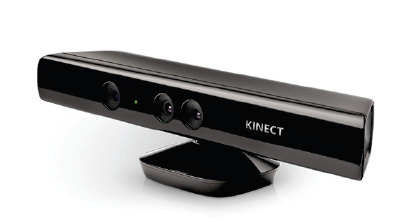
\includegraphics[width=0.7\textwidth]{Kinect360.png}
	}}
	\caption{Kinect for Xbox 360 \cite{kinectComp2011}}
	\label{fig:kinect360}
\end{figure}

\begin{itemize}
	\item First Generation Kinect 
	\item Kinect Version 1 (v1)
	\item Xbox Kinect 360 
\end{itemize} 

\paragraph{Kinect for Xbox One}
The second generation Kinect was launched in 2013. It was released with the Xbox One gaming console and is, thus, officially called the Kinect for Xbox One. \cite{kinectComp2011} A picture can be seen in Figure \ref{fig:kinectOne}. It is also referred to by different names, which are listed below for completeness:

\begin{figure}[ht]
	\centering
	{%
		\setlength{\fboxsep}{0pt}%
		\setlength{\fboxrule}{0.5pt}%
		\fbox{
			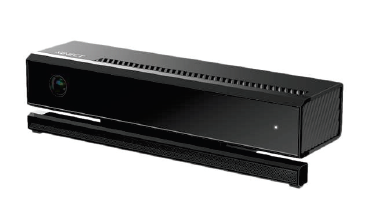
\includegraphics[width=0.7\textwidth]{KinectOne.png}
	}}
	\caption{Kinect for Xbox One \cite{kinectComp2011}}
	\label{fig:kinectOne}
\end{figure}

\begin{itemize}
	\item Second Generation Kinect 
	\item Kinect Version 2 (v2)
	\item Xbox Kinect One 
\end{itemize} 

\paragraph{Kinect for Windows}
For each generation of Kinect for Xbox released, a Kinect for Windows was released. The version numbers correlate (I.e. The Kinect for Windows also has a v1 and v2). Kinect for Windows was created to be used by a computer whereas the Kinect for Xbox to be used by the console. They are, however, functionally identical and thus, a Kinect for Xbox can be "converted" to a  Kinect for Windows by using a USB adapter. The only difference with this is that the Kinect for Windows supports "Near Mode" whereas a Kinect for Xbox used with an adapter does not. ("Near Mode" will be explained further in Section \ref{depthRange})

\paragraph{Kinect Used}
In this project, the Kinect for Xbox 360 with a USB adapter was used for development. Further reasons for this component choice is given in Section \hl{(Component Selection)}

\subsubsection{Components and Specifications} \label{kinectCompSpecs}
The Kinect for Windows (Kinect for Xbox 360 with a USB adapter) consists of a stand and a housing for the sensing components. Between the housing and a stand is a motor that is able to adjust the vertical tilt of the housing. The Kinect is able to achieve a maximum viewing angle of $43^{\circ}$ vertical by $57^{\circ}$ horizontal. It also has a vertical tilt range of $\pm27^{\circ}$. \cite{msdnKinectSpecs2017}

The housing contains the following main components:

\begin{itemize}
	\item An RGB Camera or Colour Sensor
	\item An IR Emitter
	\item An IR Depth Sensor
	\item A Microphone Array
	\item A 3-axis Accelerometer
\end{itemize}

The configuration of the stand, housing and internal components can be seen in Figure \ref{fig:kinectComponents}. A more detailed explanation of each of the components necessary for this project is included below:

\begin{figure}[ht]
	\centering
	{%
		\setlength{\fboxsep}{0pt}%
		\setlength{\fboxrule}{0.5pt}%
		\fbox{
			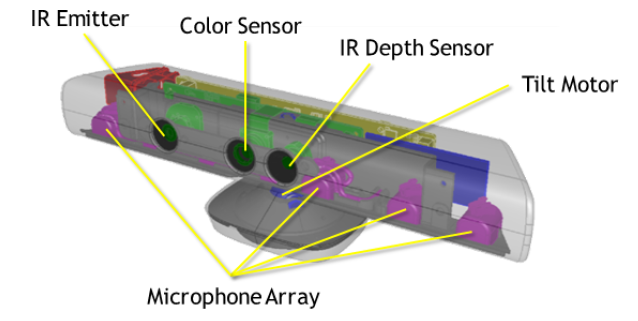
\includegraphics[width=0.7\textwidth]{Kinect360Components.png}
	}}
	\caption{Internal component layout of the Kinect for Xbox 360 \cite{msdnKinectSpecs2017}}
	\label{fig:kinectComponents}
\end{figure}

\paragraph{Colour Sensor}
The RGB camera has a maximum resolution of 1280 x 960 pixels. Each pixel is able to store red, green and blue data, allowing the camera to capture a colour image. \cite{msdnKinectSpecs2017}

\paragraph{Depth Sensor}
The depth sensor is made up of an infrared (IR) Emitter and an IR depth sensor. The emitter projects infrared light beams across the entire field of view of the Kinect. These beams hit various surfaces across the field of view and are reflected back at the Kinect. The IR depth sensor detects these reflected beams and converts them into depth data indicating the distance between the Kinect and a particular object. The collection and processing of all the reflected beams enables the Kinect to produce depth images with a maximum resolution of 640 x 480 depth image pixels. \cite{msdnKinectSpecs2017} An extension on the depth sensor is provided in the section below if more information on the intricacies of the depth sensor is required:

\subparagraph{Extension on Depth Sensor}
The depth sensor relies on a principle known as structured light. The IR emitter projects a light pattern at a wavelength of 830 nm that form an image of pseudo-random located dots. The IR depth sensor, which is an IR video-camera, also runs on a wavelength of 830 nm and can detect the light pattern. The Kinect also possesses a reference pattern that displays the light pattern at a fixed distance. This pattern is used for calibration and is used to determine depth by comparing the reflected light pattern detected with the reference pattern. \cite{kinectComp2011} This is illustrated in Figure \ref{fig:depthRefPattern}.

\begin{figure}[ht]
	\centering
	{%
		\setlength{\fboxsep}{0pt}%
		\setlength{\fboxrule}{0.5pt}%
		\fbox{
			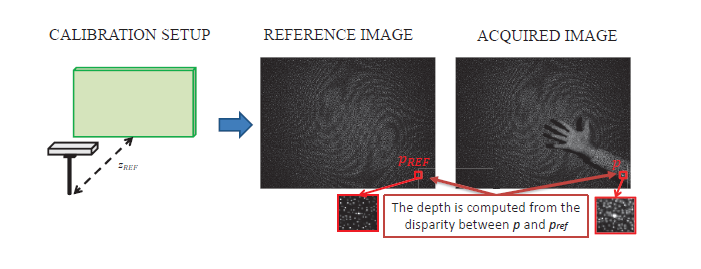
\includegraphics[width=0.7\textwidth]{depthSensorReferencePattern.png}
	}}
	\caption{An illustration of the process used by the depth sensor to determine depth by comparing the reference image to the detected one. \cite{kinectComp2011}}
	\label{fig:depthRefPattern}
\end{figure}

\subsubsection{Coordinate Spaces} \label{kinectCoordinateSpaces}
The Kinect is able to stream 3 types of data - colour, depth and skeleton data. This streamed data is available in the form of data frames that occur one at a time. The Kinect API also provides functionality that converts data between the different spaces. \cite{msdnCoSpaces2017} The sections below will elaborate on each of the spaces and will conclude with a synopsis of the conversion functionality available:

\paragraph{Colour Space}
The colour sensor is able to produce frames at a rate of 30 frames per second (fps). \cite{msdnKinectSpecs2017} Each frame captured consists of the colour image of everything inside the field of view of the colour sensor. The frame is made of pixels. As mentioned in \ref{kinectCompSpecs}, these pixels hold red, blue and green data. The number of pixels in the image depends on the resolution selected and each pixel is uniquely identified by an (x, y) coordinate. These (x, y) coordinates form the colour space. \cite{msdnCoSpaces2017}

\paragraph{Depth Space}
Similarly to the the colour sensor, the depth sensor is also able to produce frames at a rate of 30 fps. \cite{msdnKinectSpecs2017} Each frame captured also retains the information of everything in the field of view of the depth sensor and is in the form of pixels, whose size is determined by the resolution selected.  However, the difference with the depth sensor is that the data captured is a grayscale image and each pixel at a particular (x, y) coordinate, contains the Cartesian distance in millimetres from the camera plane to the nearest object, instead of red, blue and green data. The mapping of the distances to the depth space can be seen in Figure Much like the colour space, the collection of (x, y) coordinates form the depth space (I.e. The location of the depth pixels in the depth frame). The (x, y) coordinates, therefore, do not correspond to physical or Cartesian coordinates in the real world. \cite{msdnCoSpaces2017}

\begin{figure}[ht]
	\centering
	{%
		\setlength{\fboxsep}{0pt}%
		\setlength{\fboxrule}{0.5pt}%
		\fbox{
			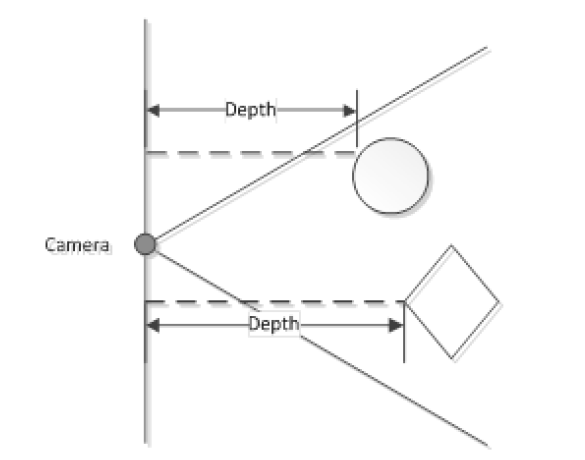
\includegraphics[width=0.7\textwidth]{distanceToDepthSpace.png}
	}}
	\caption{An illustration of the distances that stored in each depth pixel, at a particular (x, y) coordinate. \cite{msdnDepthCamKinect2017}}
	\label{fig:distanceToDepthSpace}
\end{figure}

\subparagraph{Range} \label{depthRange}
The depth sensor has two ranges - default and near range. The default range is available for both the Kinect for Windows and the Kinect for Xbox. However, as mentioned above, the near range is not available in the Kinect for Xbox. Therefore, the Kinect for Xbox use with a USB adapter will still still not have near range capabilities. The distances associated with the two ranges can be seen in Figure \ref{fig:depthSensorRanges}.

\begin{figure}[ht]
	\centering
	{%
		\setlength{\fboxsep}{0pt}%
		\setlength{\fboxrule}{0.5pt}%
		\fbox{
			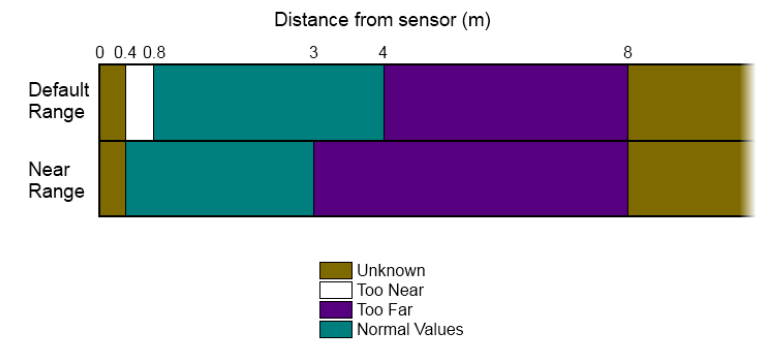
\includegraphics[width=0.7\textwidth]{depthSensorRanges.png}
	}}
	\caption{An illustration of the distances ranges for the default range and near range modes of the Kinect. \cite{msdnCoSpaces2017}}
	\label{fig:depthSensorRanges}
\end{figure}

\subparagraph{Depth Data Storage}
As mentioned above, the depth data stored in each pixel contains the distance from the depth sensor to the nearest object in millimetres. Each pixel is made up of 11 bits of information. The 3 least significant bits contain the player index and the remaining 8 bits contain the distance. \cite{msdnDepthCamKinect2017} The player index will be explained in Section \ref{kinectSkelTracking}. 

Also, as seen in Figure \ref{fig:depthSensorRanges}, there are regions of depth data in which they are classified as out of range. If a piece of depth data falls into these ranges, they are given a special value. \cite{msdnCoSpaces2017} These values are listed below:

\begin{itemize}
	\item Too Near - 0x0000
	\item Too Far - 0x0FFF
	\item Unknown - 0x1FFF
\end{itemize}  

\paragraph{Skeleton Space}
A frame of skeleton data is produced by processing a depth frame at runtime. If a person is visible in the depth sensor, skeleton data will be generated that contains 3D position data for their skeleton. Up to two human skeletons can be tracked. (Tracking is further explained in Section \ref{kinectSkelTracking}). For a tracked skeleton, all position data for their skeleton and joints are represented as 3D coordinates - (x, y, z). These coordinates are expressed in metres. The axes used to define this coordinate system is seen in Figure \ref{fig:skelSpaceAxes}. In this coordinate system, the position of the Kinect defines the origin with the positive z-axis extending in the direction the Kinect is pointing. The positive x-axis extends to the left of the Kinect and the positive y-axis extends upwards. \cite{msdnCoSpaces2017}

\begin{figure}[ht]
	\centering
	{%
		\setlength{\fboxsep}{0pt}%
		\setlength{\fboxrule}{0.5pt}%
		\fbox{
			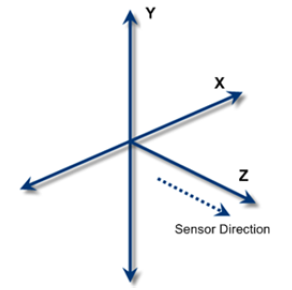
\includegraphics[width=0.7\textwidth]{skeletonSpaceAxes.png}
	}}
	\caption{An illustration of the axes used for skeleton space. \cite{msdnCoSpaces2017}}
	\label{fig:skelSpaceAxes}
\end{figure}

\subparagraph{Mirroring}
During generation of a human skeleton, the skeleton system mirrors the tracked user. This means that the left and right sides of the skeleton are inverted. This also implies that the direction of a person facing the Kinect is considered to be the -z direction. \cite{msdnCoSpaces2017}

\hl{(Clipping Paragraph - Maybe)}

\paragraph{Conversion}
Skeleton position data holds 3D positions and as such, can be thought of as real world positions. For colour and depth data, these real world positions are mapped to 2D planes. Therefore, there is a relation between the different spaces. \cite{nonContact2017} This can be seen in Figure \ref{fig:spaceConversion}. However, depth data and colour data do not always map to the same (x, y) coordinate and thus a conversion must also occur between them. \cite{msdnDepthCamKinect2017} Fortunately, these functionality for conversion between the different spaces is provided in the Kinect for Windows SDK. A link to the documentation can be seen in Section \hl{(Code documentation)}.

\begin{figure}[ht]
	\centering
	{%
		\setlength{\fboxsep}{0pt}%
		\setlength{\fboxrule}{0.5pt}%
		\fbox{
			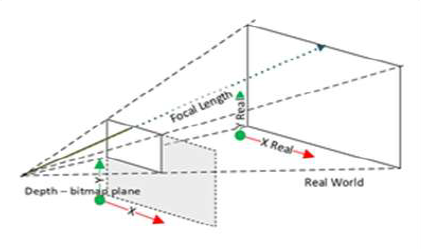
\includegraphics[width=0.7\textwidth]{spaceConversion.png}
	}}
	\caption{An illustration of the relation between the coordinate spaces for colour, depth and skeleton data. \cite{nonContact2017}}
	\label{fig:spaceConversion}
\end{figure}

\subsubsection{Skeleton Tracking} \label{kinectSkelTracking}
An inbuilt functionality of the Kinect is skeletal tracking. The skeleton system uses the depth sensor and allows the Kinect to recognise different people in its field of view and follow their actions. The Kinect can recognise up to six people in its field of view at a given time and track up to two of these users in detail. For these two tracked human skeleton, their joints are also which yields information regarding their position and movement at different time intervals. \cite{msdnSkelTrack2017}

\paragraph{User Recognition}
In order to active the recognition of the Kinect's skeletal tracking system, a person needs to be in front of the sensor with their head and upper body visible. Recognition begins automatically without any specific calibration required. In terms of the orientation of the person's body, the system functions most effectively when a person is standing or sitting, and directly facing the Kinect. Sideways poses are difficult for the system to process as the there are parts of the body not visible. \cite{msdnSkelTrack2017}

\paragraph{Field of View}
In default range mode, the skeletal tacking system has the same range as the depth sensor (Data is clearly detectable between 0.8 and 4 metres). However, users will often have to use their arms and thus, the suggested practical range for effective tracking is between 1.2 and 3.5 metres. An illustration of the field of view can be seen in Figure \ref{fig:skelTrackFieldView}.

\begin{figure}[ht]
	\centering
	{%
		\setlength{\fboxsep}{0pt}%
		\setlength{\fboxrule}{0.5pt}%
		\fbox{
			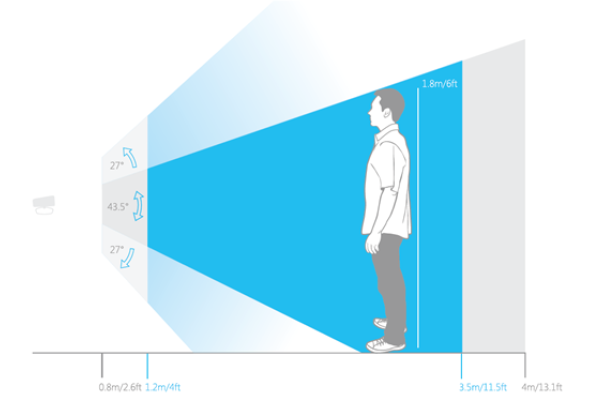
\includegraphics[width=0.7\textwidth]{skeletonTrackingFieldView.png}
	}}
	\caption{An illustration of the suggested practical field of view for effective skeletal tracking using the Kinect. \cite{msdnSkelTrack2017}}
	\label{fig:skelTrackFieldView}
\end{figure}

\paragraph{API Support}
When using the skeletal tracking system, and users are present, a skeleton frame of data is produced. This frame holds the data of up to six people in the field of view. In the frame, all skeletons of detected users can only have two states - "Tracked" or "Position Only". A "Position Only" skeleton provides information about the position of the user, but no joint information. A "Tracked" skeleton on the other hand, provides detailed information about the position, in the field of view of the sensor, of the user and twenty joints in his/her body. \cite{msdnTrackUserSkel2017} All the joints available and their positions, can be seen in Figure \ref{fig:skelAndJoints}. Each joint can also have one of three states listed below:

\begin{itemize}
	\item "Tracked" - A clearly visible joint.
	\item "Inferred" - A joint that is not clearly visible
	\item "Non-tracked" - A joint that is excluded (For example, lower joints in seated mode)
\end{itemize}

\begin{figure}[ht]
	\centering
	{%
		\setlength{\fboxsep}{0pt}%
		\setlength{\fboxrule}{0.5pt}%
		\fbox{
			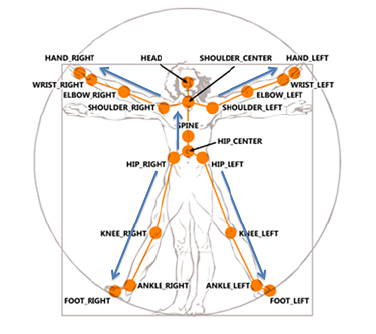
\includegraphics[width=0.7\textwidth]{skeletonAndJoints.png}
	}}
	\caption{An illustration of joints available for a "Tracked" skeleton retrieved from a skeleton frame of data. \cite{msdnTrackUserSkel2017}}
	\label{fig:skelAndJoints}
\end{figure}

As mentioned in Section \ref{litTrackSkelUsers}, full snippets of code required to track users with the Kinect skeletal tracking system, using the Kinect for Windows SDK, are provided in \cite{msdnTrackUserSkel2017}. However, a summary of the process used in C\# is given below:

\begin{enumerate}
	\item Enable skeletal tracking in an active Kinect
	\item Create an event handler to fire when a skeleton frame is ready
	\item When a skeleton frame is ready, copy the array of skeletons objects available from the frame to a new array for manipulation
	\item Loop through the array to identify the "Tracked" skeletons
	\item For a given tracked skeleton, loop through the array of joints provided for information of a single joint
	\item Utilise the information of states and/or positions of the joints and skeleton for a given application
\end{enumerate}

\paragraph{Known Errors}
Due to the structured light technology underpinning the depth sensor, there are certain environmental conditions that would affect its accuracy. Consequently, this would also affect the functioning of the skeletal tracking system. The following environmental conditions should be avoided as they significantly impair the Kinect's functioning: \cite{kinectComp2011}

\begin{itemize}
	\item The Kinect should not be used in a dark room
	\item The Kinect cannot operate with direct light shining in its direction (Should also not be used outdoors)
	\item Very reflective surfaces in the field of view of the Kinect can compromise readings	
\end{itemize} 

\hl{!!!!!!!!!!!!!!Guidelines for measurements} 

\subsubsection{Internal Process + Noise}
Middleware \cite{nonContact2017}\\
Joint Filtering\\

\subsection{Measurement}

\subsubsection{3D Space}
There are various theorems and axioms that allow for analysis of geometrical in Euclidean or three-dimensional space. One such theorem used for determining the three-dimensional distance between two points in space is the Pythagorean Theorem. Using the Cartesian coordinate system, this formula can be seen below: \cite{nonContact2017}

Let Point 1 = $(x_1, y_1, z_1)$, Point 2 = $(x_2, y_2, z_2)$ and the distance between Point 1 and Point 2 = $d$, then:\\
\begin{equation} \label{eq: distance}
d = \sqrt{(x_1 - x_2)^{2} + (y_1 - y_2)^{2} + (z_1 - z_2)^{2}}
\end{equation} 

\subsubsection{Accuracy}
When recording measurements of a physical quantity, it is often useful to understand the difference between the measured value and the actual value of the physical quantity. This difference is refereed as the measurement error or accuracy. The formula used to represent this as a percentage is seen below: \cite{nonContact2017}

Let the Measured Value = $V_{Measured}$, the Actual Value = $V_{Actual}$ and the Error = $E_\%$, then:\\
\begin{equation} \label{eq: measurementAcc}
E_\% = \frac{V_{Measured} - V_{Actual}}{V_{Actual}} \times 100
\end{equation} 

\hl{(!!!!!!!!!!!!!!!!!!!!!!!!!Uncertainty)}

\subsection{Modelling}

\subsubsection{Clothing}

\subsubsection{Ellipse}

\subsection{Clothing Industry Context} \label{clothingIndustryContext}

There currently exists 3 major channels in which clothing can be produced and sold; namely Traditional Retailers, Online Retailers and Custom Tailoring. The following paragraphs provide a short description of each of these channels:

\paragraph{Traditional Retailers}
refers to well established clothing stores presiding in areas such as shopping malls etc. These clothing stores either sell a particular brand or represent a clothing group with a collection of brands. The transaction of clothing is facilitated by a consumer visiting a store, selecting an item and purchasing it. Examples of these stores available in South Africa include:

\begin{itemize}
	\item Clothing Groups - Edgars, Truworths and Woolworths
	\item Individual Brands - Levi's, Guess and Mr Price
\end{itemize}

\paragraph{Online Retailers}
refer to either the online presence of the well established traditional retailers or of online sites that act as a distribution channel for many clothing brands. The transaction of clothing is facilitated by a consumer visiting a retailers website, selecting an item, purchasing it and either waiting for delivery or to pick up the item from a specific location. Examples of some available in South Africa include:

\begin{itemize}
	\item Traditional Retailer Online Presence - Mr Price, Forever New and Woolworths
	\item Distribution Sites - Superbalist (Child of Takealot.com) and RunwaySale
\end{itemize}

\paragraph{Custom Tailoring}
is the process whereby personalised clothing for a person based on various body measurements. Tailoring companies are normally smaller than those traditional or online retailers as they focus on a specific niche of the market. As such, they often manifest themselves in smaller "local" stores instead of large clothing brands. Obtaining custom tailored clothing is facilitated by a consumer visiting a tailor, letting the tailor measure parts of their body, waiting for the clothes to be made and finally purchasing it upon completion. 

\hl{(Get clothing references)}


\subsection{Microsoft SDK}

\subsubsection{Digital Information}

\subsubsection{Kinect Toolkit}

\paragraph{BackgroundRemoval Class}

\paragraph{Colour, Depth Class}


%Further Improvements
\subsection{Augmented Reality}
% Cellphone
% Parameter modelling
% Shadow modelling etc


\subsection{Accuracy/Other Improvement }